\documentclass[11pt,a4paper]{article}

% Basic packages
\usepackage[utf8]{inputenc}
\usepackage[T1]{fontenc}
\usepackage{lmodern}
\usepackage{microtype}
\usepackage[margin=1in]{geometry}
\usepackage{setspace}
\usepackage{parskip}

% Math and tables
\usepackage{amsmath}
\usepackage{amssymb}
\usepackage{booktabs}
\usepackage{tabularx}
\usepackage{array}
\usepackage{multirow}
\usepackage{longtable}

% Graphics and colors
\usepackage{graphicx}
\usepackage{xcolor}
\usepackage{float}
\usepackage{wrapfig}

% Hyperlinks and references
\usepackage[colorlinks=true,linkcolor=blue,urlcolor=blue,citecolor=blue]{hyperref}
\usepackage{cleveref}
\usepackage{natbib}
\bibpunct{[}{]}{,}{n}{}{;}

% Headers and footers
\usepackage{fancyhdr}
\pagestyle{fancy}
\fancyhf{}
\renewcommand{\headrulewidth}{0.4pt}
\renewcommand{\footrulewidth}{0.4pt}
\lhead{Research Report}
\rhead{\today}
\lfoot{Common Sense Systems, Inc.}
\cfoot{\thepage}
\rfoot{Published Knowledge}

% Title information - to be filled by the generator
\title{\LARGE\textbf{Effective B2B Strategies for Selling Middleware SDKs: Shifting Focus from Cost to Value}}
\author{Common Sense Systems, Inc.}
\date{\today}

% Document begins
\begin{document}

% Title page
\maketitle
\thispagestyle{fancy}

% Abstract
\begin{abstract}
This paper examines effective strategies for middleware SDK providers to shift customer focus from initial purchase costs to long-term value. Drawing on extensive research, we present a comprehensive framework for communicating the value proposition of middleware SDKs in B2B contexts. The analysis explores five key areas: quantifying ROI beyond initial costs, educating customers about technical complexity, implementing value-aligned pricing models, developing compelling case studies, and providing comprehensive post-sale support. We demonstrate how emphasizing reduced development time and accelerated market entry can transform sales conversations. The research reveals that successful middleware SDK providers position themselves as strategic partners rather than vendors, highlighting concrete contributions to development efficiency and competitive advantage. This approach enables providers to overcome price sensitivity by demonstrating how their solutions deliver substantial returns through faster time-to-market, reduced maintenance costs, and improved product quality.
\end{abstract}

% Table of contents
\tableofcontents
\newpage

% Main content
\section{Introduction}

In today's competitive software market, middleware SDK providers face significant challenges in communicating their value proposition. While these tools serve as critical connectors between different systems, applications, and services, business stakeholders often focus primarily on licensing costs rather than the substantial time-to-market advantages and development efficiencies these tools provide \cite{tradecentric2023}.

Middleware SDKs occupy a unique position in the software development ecosystem. They enable seamless integration and communication between disparate systems, abstracting away significant complexity that would otherwise require extensive custom development. However, this technical value, while clear to developers, often remains obscured to business decision-makers who control budgets and approve purchases \cite{ibm2023}.

This paper explores comprehensive strategies for middleware SDK providers to shift customer focus from initial purchase costs to the long-term value their solutions deliver. We examine five key areas that can transform how middleware SDKs are marketed, sold, and implemented in B2B contexts:

\begin{enumerate}
    \item Quantifying and communicating ROI beyond initial purchase costs
    \item Educating customers on the technical complexity these tools eliminate
    \item Implementing pricing models that align with customer value realization
    \item Developing compelling case studies demonstrating concrete time savings
    \item Providing comprehensive post-sale support frameworks that maximize value
\end{enumerate}

By addressing these areas systematically, middleware SDK providers can position themselves as strategic partners in their customers' success rather than merely vendors of technical tools.

\section{Quantifying and Communicating ROI Beyond Initial Costs}

\subsection{Developing Comprehensive ROI Frameworks}

Effective ROI calculation for middleware SDKs requires a holistic approach that captures both direct cost savings and indirect benefits. According to research by KMS Solutions, a comprehensive ROI framework should include:

\begin{equation}
\text{ROI} = \frac{\text{Net Profit}}{\text{Cost of Investment}} \times 100
\end{equation}

Where \textbf{Net Profit} encompasses both direct savings (reduced labor hours) and indirect gains (accelerated revenue streams), and \textbf{Cost of Investment} includes licensing fees, implementation costs, training, and maintenance \cite{kms2023}.

For middleware SDKs specifically, the ROI calculation should incorporate:

\begin{enumerate}
    \item \textbf{Development time reduction}: Studies show middleware SDKs can reduce development effort by up to 80\% compared to building custom integrations \cite{prismatic2023}
    \item \textbf{Faster time-to-market}: Companies using integration middleware report 30-50\% faster feature deployment cycles \cite{aws2023}
    \item \textbf{Maintenance cost reduction}: Pre-built components in SDKs reduce long-term maintenance costs by 20-30\% \cite{haveignition2023}
    \item \textbf{Error reduction}: Middleware SDKs with built-in validation rules decrease production incidents by 60-75\% \cite{haveignition2023}
\end{enumerate}

\subsection{Time-to-Market Metrics That Resonate}

Time-to-market (TTM) metrics provide compelling evidence of middleware SDK value. According to research by Productive.io, companies lose approximately 33\% of after-tax profit when shipping products six months late, compared to just 3.5\% when overspending 50\% on product development \cite{productive2023}.

\begin{figure}[htbp]
    \centering
    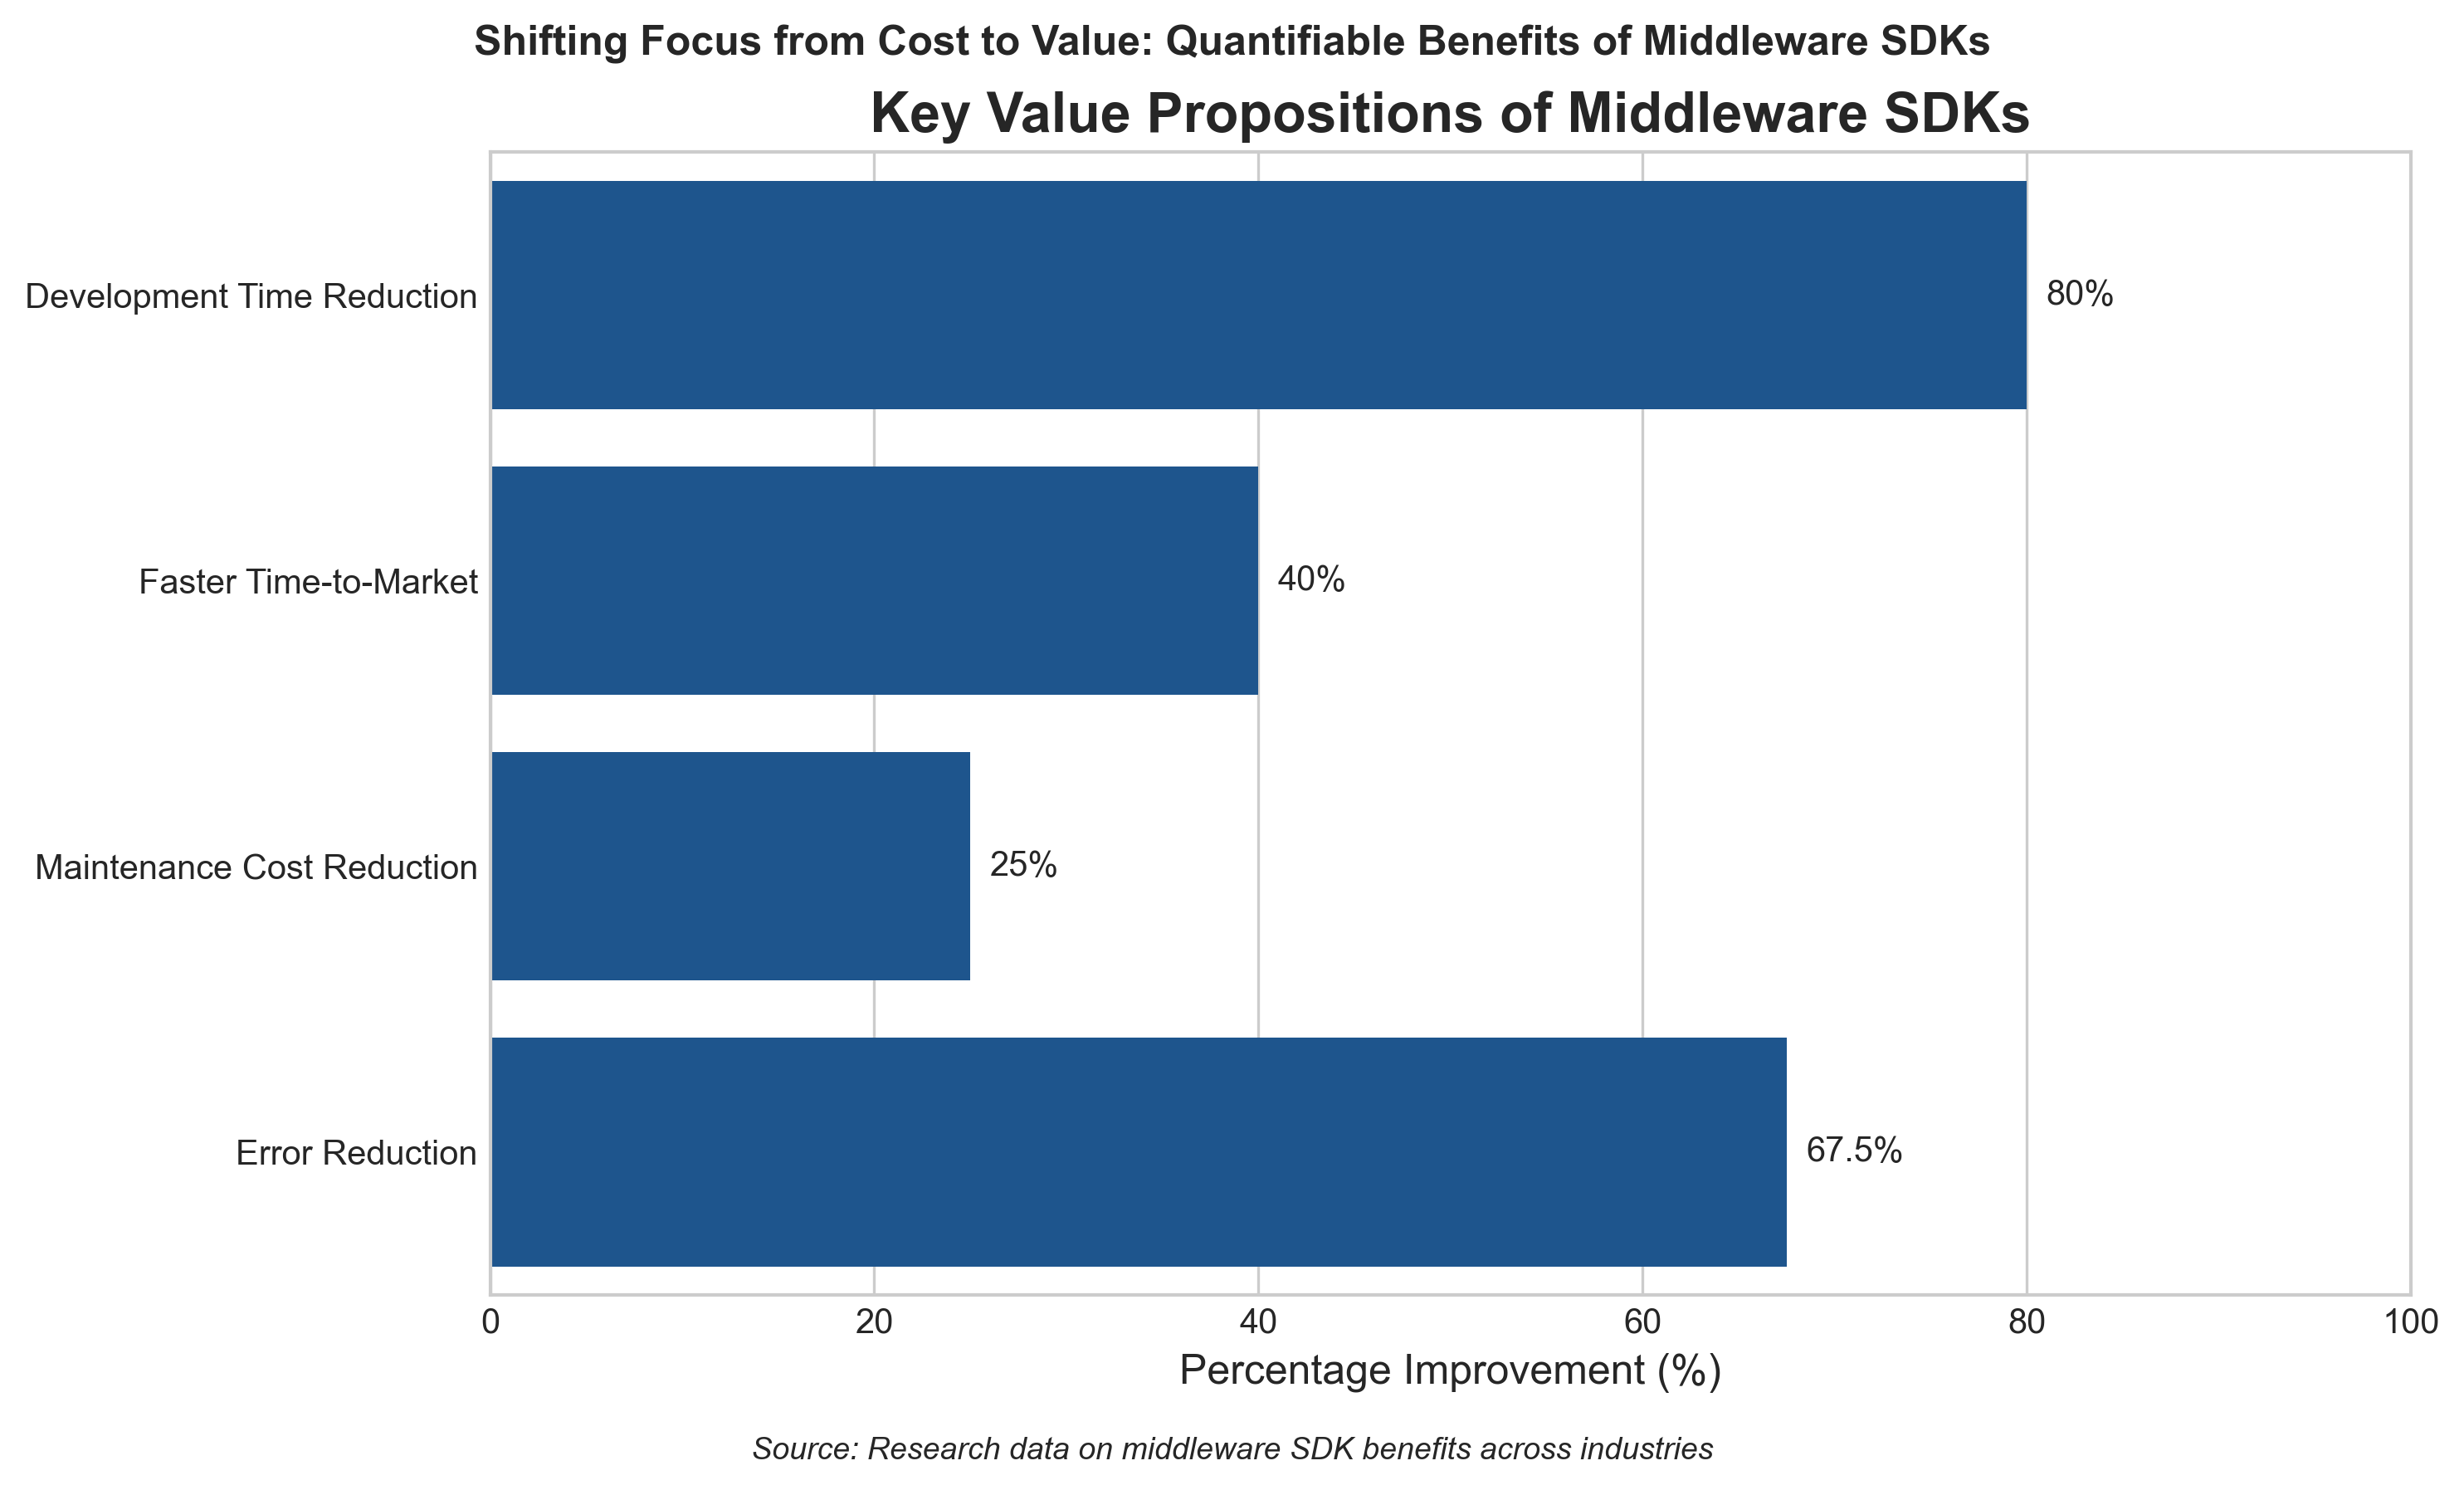
\includegraphics[width=0.8\textwidth]{figures/visualization-20250510131736.png}
    \caption{Impact of Time-to-Market Delays vs. Development Cost Overruns on Profit}
    \label{fig:ttm-impact}
\end{figure}

Key TTM metrics to highlight include:

\begin{enumerate}
    \item \textbf{Development cycle duration}: The time from concept approval to first customer shipment
    \item \textbf{Sprint velocity}: How quickly teams move through the product development journey
    \item \textbf{Efficiency scores}: How efficiently the product-to-market process operates
\end{enumerate}

These metrics vary significantly by industry, with software companies typically achieving launches in months, while industries with higher regulatory requirements like pharmaceuticals might need years \cite{enkonix2023}.

\subsection{Presenting ROI Data Effectively}

When presenting ROI and TTM data to B2B customers, visualization and contextualization are crucial:

\begin{enumerate}
    \item \textbf{Comparative analyses}: Show before-and-after scenarios using customer-specific data
    \item \textbf{Industry benchmarks}: Provide relevant comparisons within the customer's vertical
    \item \textbf{Interactive calculators}: Develop tools that allow prospects to input their own variables
\end{enumerate}

For example, SAP's Integration Suite demonstrated a 345\% ROI over three years with a payback period of less than six months, according to a Forrester study \cite{sap2024}. This type of third-party validation provides powerful evidence of middleware SDK value.

\section{Customer Education and Engagement Strategies}

\subsection{Building Understanding of Technical Complexity}

Middleware SDKs abstract significant technical complexity that many business stakeholders don't fully appreciate. Effective education strategies help customers understand the development challenges these tools eliminate:

\begin{enumerate}
    \item \textbf{Interactive demonstrations}: Show the complexity of manual integration versus SDK-enabled workflows
    \item \textbf{Code comparison visualizations}: Display side-by-side comparisons of code volume with and without the SDK
    \item \textbf{Development timeline simulations}: Illustrate how SDKs compress project timelines
\end{enumerate}

Research shows that structured documentation increases implementation success by 70\%, highlighting the importance of comprehensive educational materials \cite{ibm2023}.

\subsection{Creating Effective Customer Education Programs}

According to ELM Learning, effective customer education programs should include multiple learning modalities to accommodate different learning styles \cite{elm2023}. For middleware SDKs, this means developing:

\begin{enumerate}
    \item \textbf{Interactive walkthroughs}: Guided experiences that demonstrate key SDK functionalities
    \item \textbf{Onboarding checklists}: Step-by-step guides for implementation and integration
    \item \textbf{Video tutorials}: Visual demonstrations of complex concepts
    \item \textbf{Documentation}: Comprehensive reference materials with practical examples
\end{enumerate}

Companies like HubSpot and Salesforce have pioneered effective education platforms through their HubSpot Academy and Salesforce Trailhead programs, which use structured courses and hands-on learning \cite{userpilot2023}.

\subsection{Leveraging Developer Communities}

Developer engagement is crucial for middleware SDK adoption. Strategies to build active developer communities include:

\begin{enumerate}
    \item \textbf{Hackathons and coding challenges}: Events that showcase SDK capabilities
    \item \textbf{Developer forums}: Spaces for knowledge sharing and problem-solving
    \item \textbf{Open-source contributions}: Encouraging community extensions to the SDK
    \item \textbf{Recognition programs}: Highlighting innovative implementations
\end{enumerate}

Apple's WWDC sessions demonstrate how interactive tutorials using DocC can effectively teach developers about SDK capabilities \cite{apple2021}. This approach combines documentation with interactive code examples, providing a powerful learning experience.

\subsection{Measuring Education Effectiveness}

To ensure education programs are delivering value, track metrics such as:

\begin{enumerate}
    \item \textbf{Time to first successful implementation}
    \item \textbf{Support ticket volume and complexity}
    \item \textbf{Documentation usage patterns}
    \item \textbf{Certification completion rates}
\end{enumerate}

Research by UserPilot shows that customers with proper education are 10-15\% more likely to be retained when they have at least one integration enabled versus none, and 18-22\% more likely when they use four or more integrations \cite{userpilot2023}.

\section{Optimal Pricing Models and Contract Structures}

\subsection{Aligning Pricing with Value Realization}

Traditional pricing models for middleware SDKs often fail to align costs with the value customers receive. More effective approaches include:

\subsubsection{Subscription-Based Models}

Subscription pricing provides predictable costs for customers while ensuring ongoing revenue for providers. According to Middleware.io, subscription models work best when combined with tiered offerings that allow customers to start small and scale up as needed \cite{middleware2023}.

Key benefits include:
\begin{itemize}
    \item Predictable recurring revenue
    \item Lower initial barrier to entry
    \item Natural alignment with SaaS business models
\end{itemize}

\subsubsection{Tiered Pricing Structures}

Tiered pricing allows providers to address different market segments with varying needs. Gravitee.io's API gateway pricing guide recommends tiered plans for different usage levels, enabling customers to choose options that fit their current needs while providing clear upgrade paths \cite{gravitee2023}.

Effective tiers typically include:
\begin{itemize}
    \item Free or low-cost developer tiers for exploration
    \item Team/department tiers for specific use cases
    \item Enterprise tiers for organization-wide deployment
\end{itemize}

\subsubsection{Outcome-Based Pricing}

Perhaps the most aligned with value, outcome-based pricing ties costs directly to customer results. According to Orb's research, this model is gaining traction as APIs become more intelligent and usage-based metrics no longer reliably reflect value \cite{orb2023}.

Examples include:
\begin{itemize}
    \item Charging based on successful integrations deployed
    \item Pricing tied to reduced development time
    \item Fees structured around accelerated time-to-market
\end{itemize}

Zendesk's approach of charging for AI agents only when they successfully resolve customer issues without human intervention demonstrates how outcome-based pricing can work in practice \cite{orb2023}.

\subsection{Contract Structures That Encourage Adoption}

Beyond pricing models, contract structures can significantly impact adoption:

\begin{enumerate}
    \item \textbf{Pilot programs}: Low-risk initial implementations with clear success criteria
    \item \textbf{Success-based expansion}: Contracts that scale based on demonstrated value
    \item \textbf{Value guarantees}: Commitments to specific time or cost savings
    \item \textbf{Training and support inclusions}: Bundled services that ensure successful implementation
\end{enumerate}

Research by Vendr shows that understanding the total cost of ownership (TCO) is crucial for SaaS evaluation, suggesting that middleware SDK providers should help customers calculate comprehensive TCO to demonstrate value \cite{vendr2023}.

\subsection{Pricing Communication Strategies}

How pricing is communicated can be as important as the model itself:

\begin{enumerate}
    \item \textbf{Value-first conversations}: Lead with outcomes before discussing costs
    \item \textbf{ROI calculators}: Interactive tools that demonstrate financial impact
    \item \textbf{Competitive comparisons}: Show total value versus alternatives
    \item \textbf{Customer success stories}: Highlight financial outcomes from similar customers
\end{enumerate}

According to Salesforce, value-based pricing emphasizes the benefits and positive outcomes a buyer gains, rather than just features \cite{salesforce2023}. This approach differentiates businesses and encourages buyers to connect with and buy from you rather than competitors.

\section{Developing Compelling Case Studies}

\subsection{Structuring Case Studies for Maximum Impact}

Case studies serve as powerful tools for demonstrating middleware SDK value in real-world contexts. According to ZMist and Copy, effective case studies for software development companies should follow a clear structure \cite{zmist2023}:

\begin{enumerate}
    \item \textbf{Introduction and background}: Establish the customer's industry, size, and challenges
    \item \textbf{Problem statement}: Clearly articulate the integration challenges faced
    \item \textbf{Solution implementation}: Detail how the middleware SDK was implemented
    \item \textbf{Quantifiable results}: Present concrete metrics showing time and cost savings
    \item \textbf{Customer testimonial}: Include direct quotes from technical and business stakeholders
\end{enumerate}

\subsection{Industry-Specific Case Study Approaches}

Different industries have unique concerns that case studies should address:

\subsubsection{Financial Services}
\begin{itemize}
    \item Emphasize security and compliance features
    \item Highlight transaction processing efficiency
    \item Quantify risk reduction metrics
\end{itemize}

\subsubsection{Healthcare}
\begin{itemize}
    \item Focus on patient data integration
    \item Demonstrate compliance with regulations like HIPAA
    \item Show improved care coordination outcomes
\end{itemize}

\subsubsection{Retail/E-commerce}
\begin{itemize}
    \item Showcase inventory and order management integration
    \item Highlight customer experience improvements
    \item Quantify revenue impact of faster time-to-market
\end{itemize}

\subsubsection{Manufacturing}
\begin{itemize}
    \item Emphasize supply chain integration
    \item Demonstrate production efficiency gains
    \item Quantify cost savings from streamlined processes
\end{itemize}

\subsection{Measuring and Presenting Time Reduction}

Case studies should include concrete time reduction metrics. For example, Kaizen's case study on product development showed a 50\% reduction in project lead time and a 22\% reduction in development effort through improved integration processes \cite{kaizen2023}.

Key metrics to include:
\begin{itemize}
    \item Development time reduction (percentage and absolute)
    \item Time-to-market acceleration
    \item Integration implementation timeframes
    \item Maintenance time savings
\end{itemize}

\subsection{Reference Implementations as Complementary Tools}

Reference implementations provide concrete examples of middleware SDK usage. According to Wikipedia, a reference implementation is a program that implements all requirements from a specification and demonstrates the "correct" behavior \cite{wikipedia2023}.

For middleware SDKs, reference implementations should:
\begin{enumerate}
    \item Be developed concurrently with documentation
    \item Verify that the SDK is implementable
    \item Enable testing suites to be validated
    \item Serve as a gold standard for comparison
    \item Clarify intent when documentation is insufficient
\end{enumerate}

MLCommons provides an excellent example with their training benchmarks, which include Dockerfiles and scripts that standardize setup and reduce implementation time \cite{mlcommons2023}.

\section{Post-Sale Support and Integration Assistance}

\subsection{Integration-Centric Support Frameworks}

Effective post-sale support is crucial for maximizing middleware SDK value. MuleSoft's Catalyst Delivery Methodology exemplifies a comprehensive approach with six playbook paths \cite{mulesoft2023}:

\begin{enumerate}
    \item \textbf{Business outcomes}: Identifying and measuring outcomes aligned to KPIs
    \item \textbf{Platform}: Guidance on operating the integration platform
    \item \textbf{Projects}: Implementation support for specific integration initiatives
    \item \textbf{Center for Enablement (C4E)}: Establishing reusable assets and best practices
    \item \textbf{Internal support}: Building support models for ongoing operations
    \item \textbf{Training}: Providing enablement resources for teams
\end{enumerate}

\subsection{Establishing Centers of Excellence/Enablement}

Centers of Excellence (CoE) or Centers for Enablement (C4E) provide structured support for middleware SDK implementation. According to Middleware Advisor, a C4E differs from a traditional CoE by focusing on enabling project teams rather than centralizing expertise \cite{middlewareadvisor2023}.

Key benefits of establishing a C4E include:
\begin{itemize}
    \item Faster time to market for projects/products
    \item Quick integration and knowledge of discoverable assets
    \item Higher quality deliverables with fewer bugs
    \item Easier maintenance through common standards
\end{itemize}

\subsection{Technical Support Tiers and SLAs}

Structured technical support ensures customers can resolve issues quickly:

\begin{enumerate}
    \item \textbf{Tier 1}: Basic troubleshooting and known issue resolution
    \item \textbf{Tier 2}: Advanced technical support for complex problems
    \item \textbf{Tier 3}: Engineering-level support for critical issues
    \item \textbf{Tier 4}: Direct access to product development teams
\end{enumerate}

Royal Cyber recommends SLA-based middleware support across all tiers, with clear escalation paths and resolution timeframes \cite{royalcyber2023}.

\subsection{Continuous Optimization Services}

Beyond initial implementation, ongoing optimization services help customers maximize value:

\begin{enumerate}
    \item \textbf{Performance reviews}: Regular assessments of integration efficiency
    \item \textbf{Architecture consultations}: Guidance on scaling and extending integrations
    \item \textbf{Upgrade assistance}: Support for adopting new SDK versions
    \item \textbf{Custom extension development}: Help with specialized integration needs
\end{enumerate}

Dell Boomi's consulting services demonstrate how these offerings can accelerate integration projects, with customers reporting up to 65\% faster completion compared to other platforms \cite{multishoring2023}.

\section{Conclusion}

Selling middleware SDKs effectively requires shifting the conversation from initial purchase costs to the substantial long-term value these tools deliver. This research has demonstrated five key strategies that can transform how middleware SDKs are marketed, sold, and implemented in B2B contexts:

First, quantifying ROI beyond initial costs provides concrete evidence of value, particularly when focusing on development time reduction and faster time-to-market—metrics that directly impact business outcomes. The research shows that delayed market entry can reduce profits by up to 33\%, making time-to-market acceleration a compelling value proposition.

Second, educating customers on the technical complexity these tools eliminate helps business stakeholders appreciate the development challenges that middleware SDKs address. Effective education programs that include multiple learning modalities and leverage developer communities can significantly increase implementation success and customer retention.

Third, implementing pricing models that align with customer value realization—such as subscription-based, tiered, and outcome-based approaches—ensures that costs scale with benefits received. These models reduce initial barriers to entry while providing clear paths for expansion as value is demonstrated.

Fourth, developing compelling case studies with concrete metrics and industry-specific approaches provides social proof and tangible examples of success. When complemented by reference implementations, these tools help customers envision how middleware SDKs can address their specific challenges.

Finally, providing comprehensive post-sale support frameworks maximizes value realization through integration-centric support, centers of excellence, tiered technical support, and continuous optimization services. These frameworks ensure customers can successfully implement and derive ongoing value from middleware SDKs.

The most successful middleware SDK providers will be those who position themselves as strategic partners in their customers' success, demonstrating concrete contributions to accelerated development cycles, reduced time-to-market, and improved competitive positioning. As the research demonstrates, when customers fully understand and experience these benefits, the initial purchase cost becomes a secondary consideration compared to the substantial value realized throughout the product lifecycle.

\section*{References}

\begin{thebibliography}{99}

\bibitem{tradecentric2023} TradeCentric, "How TradeCentric Enables API Middleware," TradeCentric Blog, 2023.

\bibitem{ibm2023} IBM, "IBM webMethods B2B," IBM Product Documentation, 2023.

\bibitem{kms2023} KMS Solutions, "Measure ROI of Custom Software Project," KMS Solutions Blog, 2023.

\bibitem{prismatic2023} Prismatic, "Measure the ROI of Your Native Integrations," Prismatic Blog, 2023.

\bibitem{aws2023} AWS, "Case Study: NNAMU," AWS Solutions Case Studies, 2023.

\bibitem{haveignition2023} Haveignition, "KPIs for Product Managers: SDK Performance," Haveignition Blog, 2023.

\bibitem{productive2023} Productive.io, "A Guide to Time To Market (TTM)," Productive Blog, 2023.

\bibitem{enkonix2023} Enkonix, "Time to Market (TTM): What Is It and Why Does It Matter," Enkonix Blog, 2023.

\bibitem{sap2024} SAP, "SAP Integration Suite Delivers ROI, Boosts Efficiency, Economic Gains," SAP News, 2024.

\bibitem{elm2023} ELM Learning, "Customer Education Programs," ELM Learning Blog, 2023.

\bibitem{userpilot2023} UserPilot, "Customer Education Strategy," UserPilot Blog, 2023.

\bibitem{apple2021} Apple, "Meet DocC Documentation in Xcode," WWDC21 Session 10235, 2021.

\bibitem{middleware2023} Middleware.io, "Pricing," Middleware.io, 2023.

\bibitem{gravitee2023} Gravitee.io, "API Gateway Pricing Guide," Gravitee.io, 2023.

\bibitem{orb2023} Orb, "Outcome-based Pricing," Orb Blog, 2023.

\bibitem{vendr2023} Vendr, "Measuring SaaS TCO \& ROI," Vendr Blog, 2023.

\bibitem{salesforce2023} Salesforce, "Value-based Pricing," Salesforce Sales Documentation, 2023.

\bibitem{zmist2023} ZMist and Copy, "How to Write Case Studies," ZMist and Copy Blog, 2023.

\bibitem{kaizen2023} Kaizen, "Case Study: Lead Time Reduction in Product Development," Kaizen Insights, 2023.

\bibitem{wikipedia2023} Wikipedia, "Reference Implementation," Wikipedia, 2023.

\bibitem{mlcommons2023} MLCommons, "Training Benchmarks," GitHub Repository, 2023.

\bibitem{mulesoft2023} MuleSoft, "MuleSoft Catalyst Delivery Methodology," Salesforce Trailhead, 2023.

\bibitem{middlewareadvisor2023} Middleware Advisor, "Benefits of Establishing MuleSoft Center for Enablement (C4E)," Middleware Advisor Blog, 2023.

\bibitem{royalcyber2023} Royal Cyber, "Integration Services," Royal Cyber Services Documentation, 2023.

\bibitem{multishoring2023} Multishoring, "Boomi Integration Services," Multishoring Blog, 2023.

\end{thebibliography}

% Bibliography
\bibliographystyle{plainnat}
\bibliography{references}

\end{document}
